%%%%%%%%%%%%%%%%%%%%%%%%%%%%%%%%%%%%%%%%%%%%%%%%%%%%%%%%%%%%%%%%%%%%%%%%%%%%%%%%%%%%%%%
%     <-- выше автоматическая преамбула  |  пользовательская преамбула ниже --->      %
%%%%%%%%%%%%%%%%%%%%%%%%%%%%%%%%%%%%%%%%%%%%%%%%%%%%%%%%%%%%%%%%%%%%%%%%%%%%%%%%%%%%%%%

%%% Работа с русским языком
\usepackage{cmap}					    % поиск в PDF
\usepackage{mathtext} 				% русские буквы в формулах

% Для разметки слайдов и картинок
\usepackage{tikz}
\usepackage{animate}

% Для двойных прямых кавычек в Verbatim (не работает почему-то)
\usepackage{upquote}

% % Работа с прочими шрифтами
% \usepackage{fontspec}      %% УЖЕ ЗАГРУЖЕН В ПРЕАМБУЛЕ подготавливает загрузку шрифтов Open Type, True Type и др.
\setmainfont{Times New Roman} %% задаёт основной шрифт документа
\setsansfont{Microsoft Sans Serif} %% задаёт шрифт без засечек
\setmonofont[Scale=0.7]{DejaVu Sans Mono} %% моноширинный шрифт\

%% математический шрифт
\setmathfont[version=Cambria]    {Cambria Math}
\setmathfont[version=LatinModern]{Latin Modern Math}
\mathversion{Cambria}

% Межстрочный интервал в verabtim
\makeatletter
\def\verbatim@font{\linespread{0.7}\normalfont\ttfamily}
\makeatother

% Межабзацный интервал в columns
\makeatletter
\newcommand{\@minipagerestore}{\setlength{\parskip}{4pt plus 2pt minus 1pt}}
\makeatother

% \usepackage{hyperref} %% УЖЕ ЗАГРУЖЕН В ПРЕАМБУЛЕ
\definecolor{links}{HTML}{2A1B81}
\hypersetup{colorlinks=true,linkcolor=,urlcolor=links,pdfview=FitH,pdfpagelayout=SinglePage, unicode=true,breaklinks=true}

% Тильда в тексте
\newcommand{\mytilde}{\char`~\:}
% argmin и argmax
\DeclareMathOperator*{\argmax}{argmax}
\DeclareMathOperator*{\argmin}{argmin}

% Более простой ввод команд для двухколоночной верстки
\newcommand{\columnsbegin}{\vspace{-0.5\baselineskip}\begin{columns}[t,onlytextwidth]}
\newcommand{\columnsend}{\end{columns}}
\newcommand{\columnbegin}{\begin{column}}
\newcommand{\columnend}{\end{column}}
\newcommand{\blockbegin}{\begin{block}}
\newcommand{\blockend}{\end{block}}

% allows to add alignment keys to \includegraphics
\usepackage[export]{adjustbox}

% Работа с таблицами %%%%%%%%%%%%%%

\usepackage{adjustbox}

% Новые типы колонок для окружения tabular, чтобы можно было задавать их ширину
% Например, \begin{tabular}{ L{2.3cm} C{2cm} C{1.5cm} C{2.5cm} C{4cm}}
\usepackage{array}
\renewcommand{\arraystretch}{1.5}
\newcolumntype{L}[1]{>{\raggedright\let\newline\\\arraybackslash\hspace{0pt}}m{#1}}
\newcolumntype{C}[1]{>{\centering\let\newline\\\arraybackslash\hspace{0pt}}m{#1}}
\newcolumntype{R}[1]{>{\raggedleft\let\newline\\\arraybackslash\hspace{0pt}}m{#1}}

% Для таблиц в tabularx окружении при помощи пакета huxtable
\usepackage{tabularx}

% Прочие настройки beamer %%%%%%%%%%%%

% Цвета
% Посмотреть и конвертировать можно здесь https://convertingcolors.com/
%                       RGB                       HEX    nearest R colour
\definecolor{spbblack}{RGB}{30,30,30}           % 1e1e1e "gray12"
\definecolor{spbgrey}{RGB}{191,191,191}         % BFBFBF "gray75"
\definecolor{spbteal}{RGB}{188, 216, 221}       % BCD8DD "powderblue"
\definecolor{spblightteal}{RGB}{222,236,238}    % DEECEE "azure2"
\definecolor{spbred}{RGB}{203,55,87}            % CB3757 "maroon"
\definecolor{spbgreen}{RGB}{168,207,166}        % A8CFA6 "darkseagreen3"
\definecolor{spbdarkgreen}{RGB}{96,157,131}     % 609D83 "paleturquoise4"
\definecolor{spbblue}{RGB}{98,122,235}          % 627AEB "cornflowerblue"
\definecolor{spbdarkblue}{RGB}{24,112,184}      % 1870B8 "dodgerblue3"
\definecolor{spbviolet}{RGB}{212,207,232}       % D4CFE8
\definecolor{spbdarkviolet}{RGB}{101,118,185}   % 6576B9
\definecolor{spbyellow}{RGB}{254,192,15}        % FEC00F "darkgoldenrod1"
\definecolor{spbsteelblue}{RGB}{70,130,180}     % 4682B4 "steelblue"


% Галочка в тексте
\def\checkmark{\tikz\fill[scale=0.4](0,.35) -- (.25,0) -- (1,.7) -- (.25,.15) -- cycle;}

% Для раскраски таблиц
\usepackage{colortbl}
% переопределяем tabular с раскраской
\let\oldtabular\tabular
\let\endoldtabular\endtabular
\renewenvironment{tabular}{
\setlength\arrayrulewidth{1pt} \arrayrulecolor{white}
\rowcolors{1}{spbteal}{spblightteal}
\oldtabular}{\endoldtabular}

\usepackage{caption}
\captionsetup[table]{name=Таблица}
% переопределяем tabularx с раскраской
\let\oldtabularx\tabularx
\let\endoldtabularx\endtabularx
\renewenvironment{tabularx}{
\setlength\arrayrulewidth{1pt} \arrayrulecolor{white}
\rowcolors{1}{spbteal}{spblightteal}
\oldtabularx}{\endoldtabularx}


% Для подсветки элементов формул
\usepackage[beamer,customcolors,norndcorners]{hf-tikz}
\hfsetfillcolor{spbteal}
\hfsetbordercolor{white}

\setbeamercolor{myfootlinetext}{fg=spbgrey}
\setbeamerfont{myfootlinetext}{size=\normalsize}
% Переопределяем бимеровский footline
\setbeamertemplate{footline}{
  % \vspace{1cm}
  \usebeamercolor[fg]{myfootlinetext}
  \usebeamerfont{myfootlinetext}
  \hspace{0.5cm}\textbf{\insertpagenumber}\hfill\strut\quad
  \vspace{0.4cm}
}

% Фон слайдов
\usepackage{etoolbox}
\makeatletter
\setbeamertemplate{background canvas}{%
   \ifnumequal{\c@framenumber}{1}{%
      % First frame
      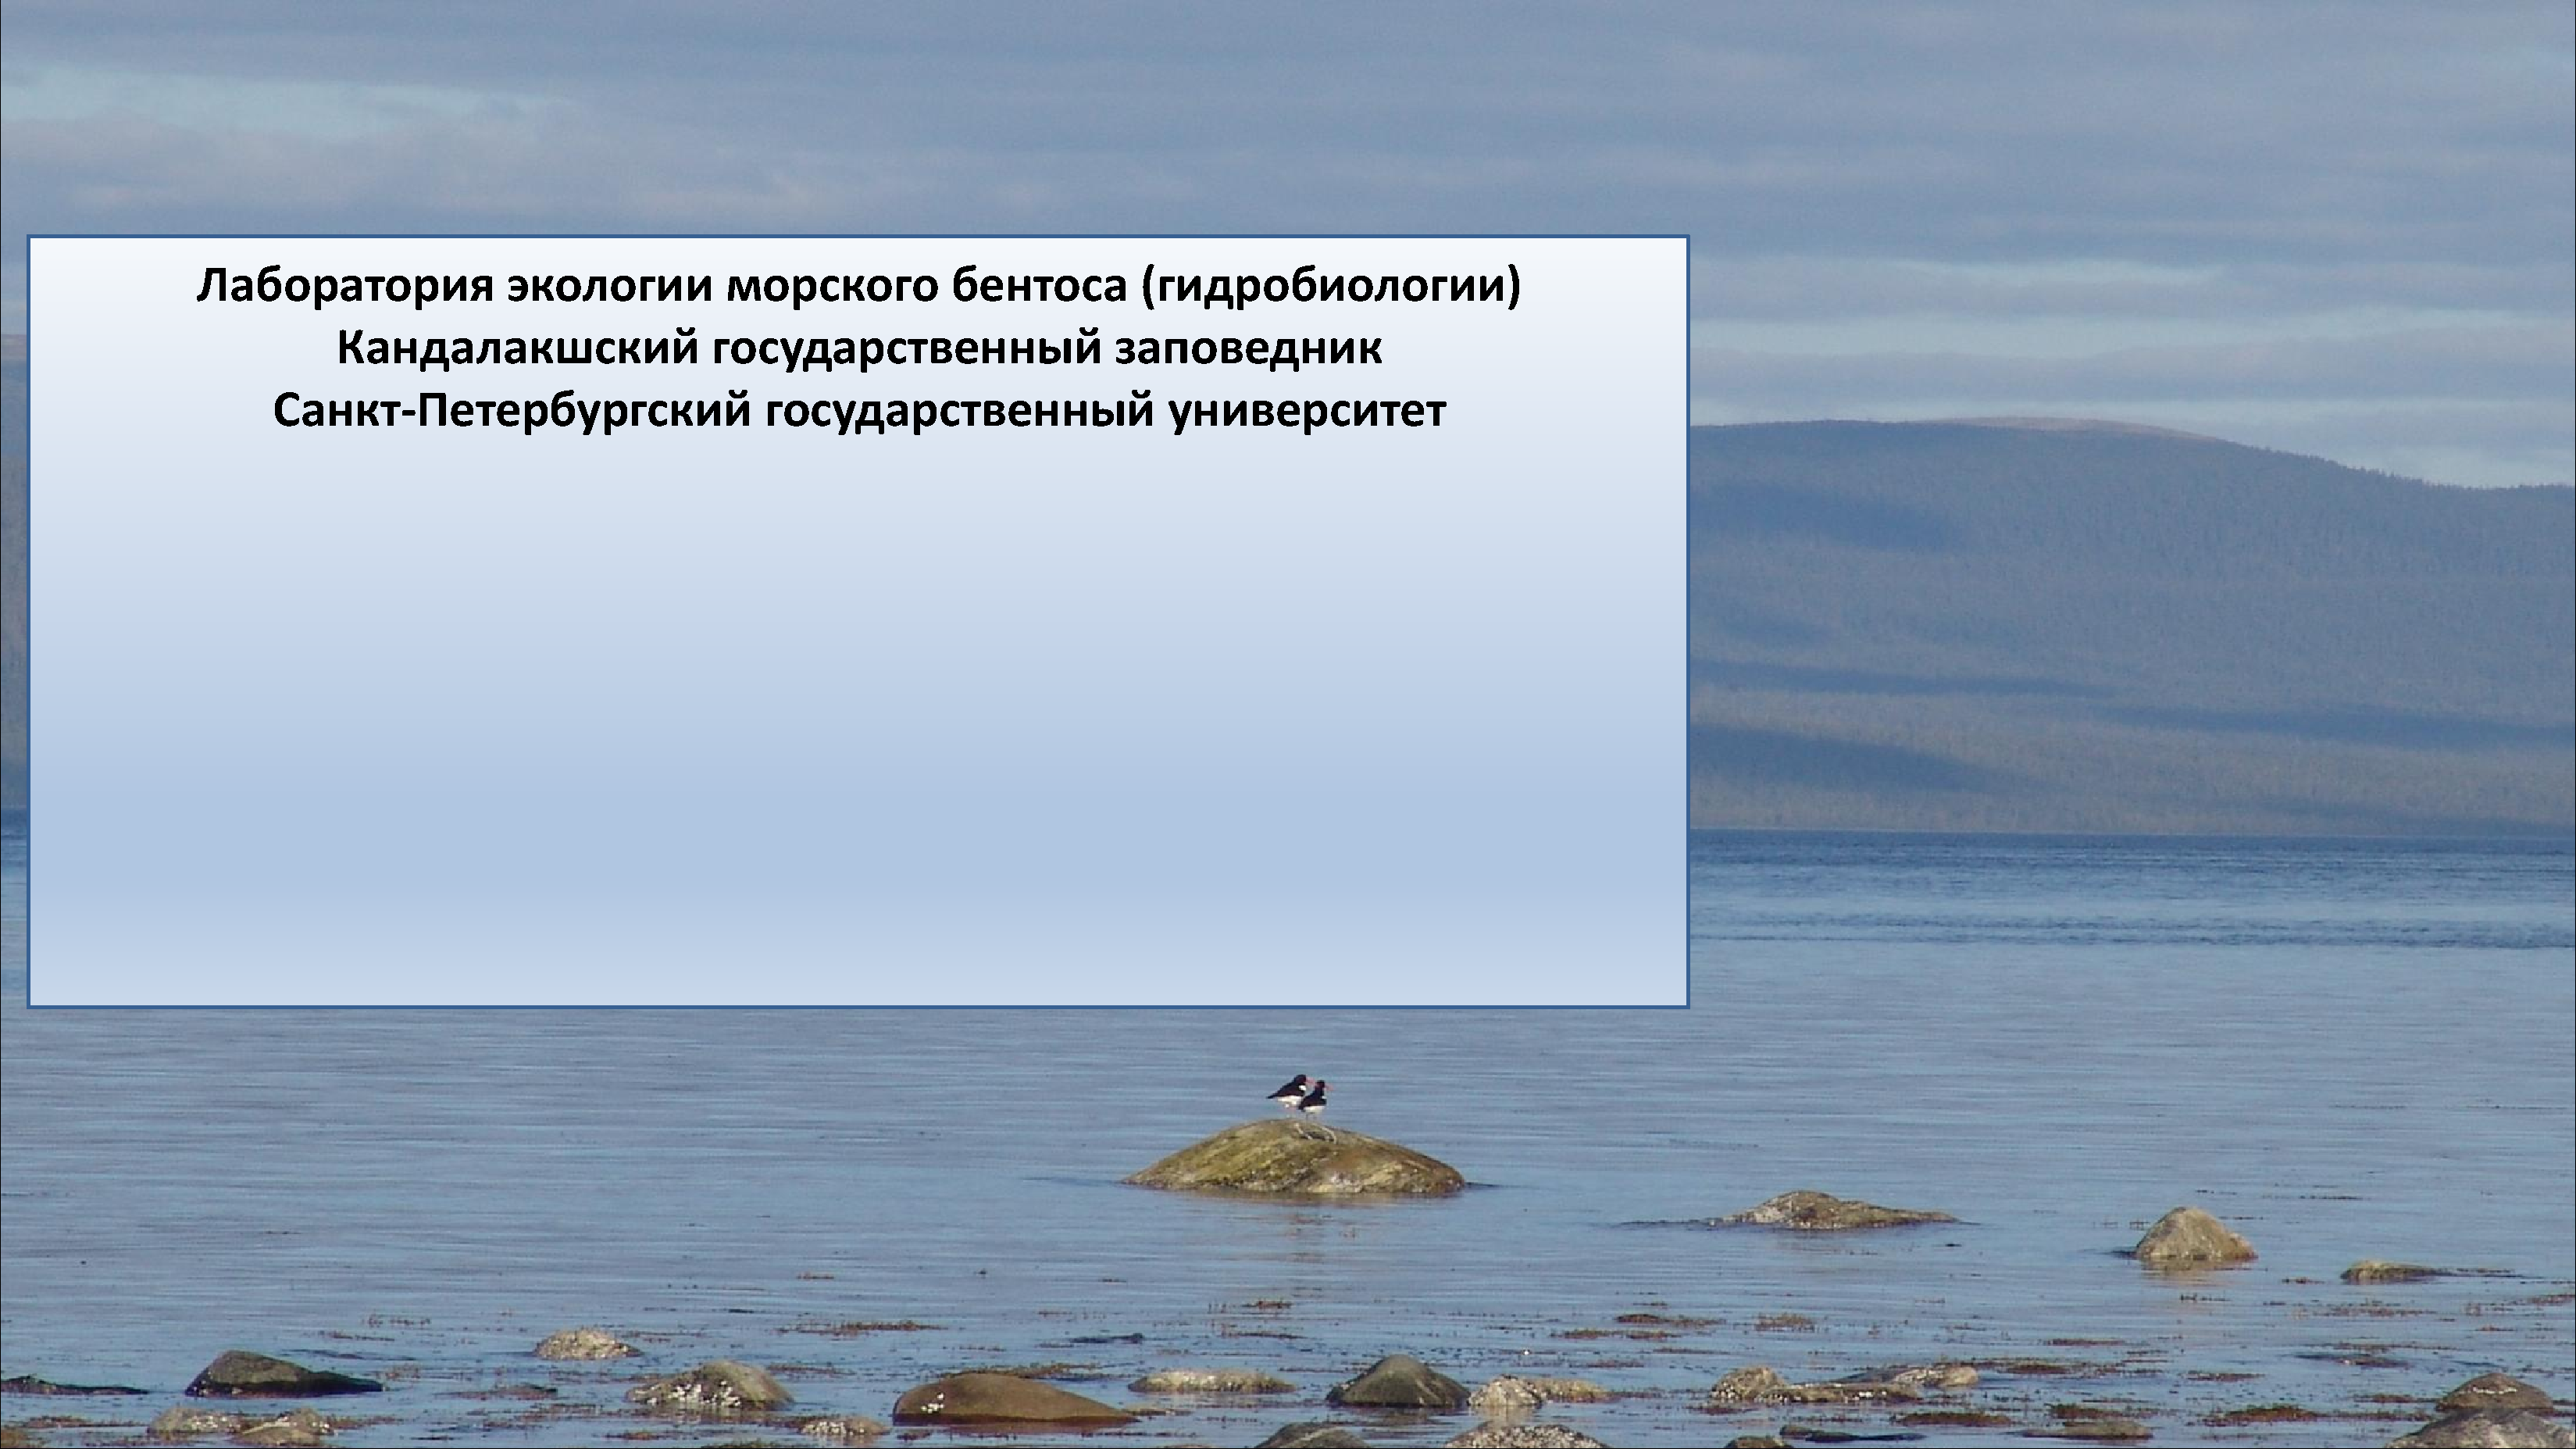
\includegraphics[width=\paperwidth,height=\paperheight]{includes/Primer_title.pdf}
   }{%
      \ifnumequal{\c@framenumber}{\inserttotalframenumber-1}{
         % Before last frame
         
\includegraphics[width=\paperwidth,height=\paperheight]{includes/Primer_sources.pdf}
      }{%
      \ifnumequal{\c@framenumber}{\inserttotalframenumber}{
         % Last frame
         
\includegraphics[width=\paperwidth,height=\paperheight]{includes/Primer_last.pdf}
      }{%
         % Other frames
         
\includegraphics[width=\paperwidth,height=\paperheight]{includes/Primer_slide.pdf}
      }%
   }%
   }%
}
\makeatother

% Разметка титульного слайда
\setbeamertemplate{title page}{%
    \begin{tikzpicture}[remember picture,overlay]
    % Заголовок
    \node[anchor=west]
    at ([yshift=-25mm,xshift=18mm]current page.north west) (title)
    {\parbox[b][1in]{0.45\paperwidth}{\raggedright%
            \usebeamerfont{title}\textcolor{spbblack}{\textbf\inserttitle}}};
    % Автор
    \node[anchor=west]
    at ([yshift=-57mm,xshift=18mm]current page.north west) (author)
    {\parbox[t][1in]{.45\paperwidth}{\raggedright%
            \usebeamerfont{author}\textcolor{spbblack}{\insertauthor}}};
    % Организация
    \node[anchor=north west]
    at ([yshift=37mm,xshift=18mm]current page.south west) (institute)
    {\parbox[t]{.45\paperwidth}{\raggedright%
            \usebeamerfont{institute}\textcolor{spbblack}{\insertinstitute}}};
    \end{tikzpicture}
}
% Заголовок на титульном слайде
\setbeamercolor{titlelike}{parent=palette primary,fg=spbblack,bg=}

% Блоки
\setbeamercolor{block title}{fg=spbblack, bg=}

% Заголовки слайдов
\setbeamercolor{frametitle}{bg=}
\setbeamertemplate{frametitle}{
  \vspace{1cm}
  \color{spbblack}\bfseries\insertframetitle%
}

% Маркеты элементов списка
\setbeamertemplate{itemize items}{\color{spbteal}\normalsize$\bullet$}


%%%%%%%%%%%%%%%%%%%%%%%%%%%%%%%%%%%%%%%%%%%%%%%%%%%%%%%%%%%%%%%%%%%%%%%%%%%%


